%!TEX program = xelatex
\documentclass[11pt,a4paper]{article}
\usepackage[utf8]{inputenc}
\usepackage[T1]{fontenc}
\usepackage{ctex}
\usepackage{authblk}
\usepackage{tikz}
\usepackage{pgfplots}
\usepackage{verbatim}
\usepackage{amsfonts}
\usepackage{amsmath}
\usepackage{amsthm}
\usepackage{indentfirst}
\usepackage{amssymb}
\usepackage{enumerate}
\setlength{\parindent}{0pt}
\usetikzlibrary{shapes,snakes}
\newcommand{\argmax}{\operatornamewithlimits{argmax}}
\newcommand{\argmin}{\operatornamewithlimits{argmin}}

\DeclareMathOperator{\col}{col}
\usepackage{booktabs}
\newtheorem{theorem}{Theorem}
\newtheorem{proposition}{Proposition}
\newtheorem{definition}{Definition}
\newtheorem{lemma}{Lemma}
\newtheorem{example}{Example}
\newtheorem{corollary}{Corollary}
\newtheorem{note}{Note}
\usepackage{graphicx}
\usepackage{geometry}
\usepackage{hyperref}
\newcommand{\code}{	exttt}
\geometry{a4paper,scale=0.8}
\title{MATH 417 Lec01-05}
\author[*]{Wenxiao Yang}
\affil[*]{Department of Mathematics, University of Illinois at Urbana-Champaign}
\date{2021}





\begin{document}
\maketitle
\tableofcontents

\newpage
\section{Function and Set}
\subsection{Function}
\noindent $A\times B=\{(a,b)|a\in A, b\in B\}$.\\
\underline{\textit{Function}} is a rule $\sigma$ that assigns an element $B$ to \textit{every} element of $A$.
\begin{equation}
    \begin{aligned}
    &\sigma:A\rightarrow B\\
    & \forall a\in A, \sigma(a)\in B.\\
    & \sigma (a)= \textit{value of } \sigma\textit{ at } a. \textit{ (the \underline{image} of $a$)}
    \end{aligned}
    \nonumber
\end{equation}
A set $C\subset B$, we call $\sigma^{-1}(C)=\{a\in A| \sigma(a)\in C\}$ as the \textit{\underline{preimage}} of $a$.\\
An element $b\in B$, we call $\sigma^{-1}(b)=\{a\in A| \sigma(a)=b \}$ as the \textit{\underline{fiber}} of $b$.\\
$A$ is the \underline{domain} of $\sigma$, $B$ is the \underline{range} of $\sigma$.

\subsubsection{Composition of functions}
$\sigma: A\rightarrow B, \tau: B\rightarrow C$. The function $\tau\circ \sigma:A\rightarrow C$ is $\forall a\in A,\ (\tau\circ \sigma)(a)=\tau( \sigma(a))$

\subsubsection{Proposition 1.1.3: Associativity of Functions}
\begin{proposition}[Proposition 1.1.3]
    $\sigma:A \rightarrow B, \tau:B \rightarrow C, \rho:C \rightarrow D$ functions then,
    \begin{equation}
        \begin{aligned}
            \rho\circ(\tau\circ\sigma)=(\rho\circ\tau)\circ\sigma
        \end{aligned}
        \nonumber
    \end{equation}
\end{proposition}
\subsubsection{Injective, surjective, bijective}
A function $\sigma:A \rightarrow B$ is called,\\
1. \textit{Injective (1 to 1)}
\begin{equation}
    \begin{aligned}
        \forall a_1,a_2\in A, \sigma(a_1)=\sigma(a_2)\Rightarrow a_1=a_2
    \end{aligned}
    \nonumber
\end{equation}
2. \textit{Surjective (onto)}
\begin{equation}
    \begin{aligned}
        \forall b\in B,\exists a\in A, s.t. \sigma(a)=b
    \end{aligned}
    \nonumber
\end{equation}
3. \textit{Bijective} (if injective and surjective)

\subsubsection{Lemma 1.1.7: 两个injective/surjective/bijective的方程的composition保留性质}
\begin{lemma}[Lemma 1.1.7]
    Suppose $\sigma:A \rightarrow B, \tau: B \rightarrow C$ are functions,\\
    If $\sigma, \tau$ are injective, then $\tau\circ\sigma$ is \textit{injective}.\\
    If $\sigma, \tau$ are surjective, then $\tau\circ\sigma$ is \textit{surjective}.\\
    If $\sigma, \tau$ are bijective, then $\tau\circ\sigma$ is \textit{bijective}.\\
\end{lemma}

\subsubsection{Proposition 1.1.8: Inverse of Function}
\begin{proposition}[Proposition 1.1.8]
    A function $\sigma:A \rightarrow B$ is a bijection if\\
    $\exists$ a function $\tau:B \rightarrow A $ such that
    \begin{equation}
        \begin{aligned}
            &\sigma\circ\tau=id_B=\textit{identity on }B(id_B(x)=x, \forall x\in B)\\
            &\tau\circ\sigma=id_A
        \end{aligned}
        \nonumber
    \end{equation}
\end{proposition}
Such $\tau$ is unique, called inverse of $\sigma$, $\tau=\sigma^{-1}$.

\subsection{Set}
\subsubsection{Well Defined Set}
\begin{definition}
    A set $S$ is \textbf{well defined} if an object $a$ is either $a\in S$ or $a\notin S$.
\end{definition}
\subsubsection{Power Set}
\begin{definition}
    For any set $A$, we denote by $\mathcal{P}(A)$ the collection of all subsets of $A$. $\mathcal{P}(A)$ is the \textbf{power set} of $A$.
\end{definition}
\subsubsection{Cardinalities of Sets, Pigeonhole Principle}
\begin{definition}
    If $A$ is a set, $|A|=$ cardinality of $A$ = $\#$ of elements
\end{definition}
$n \in \mathbb{N},|\{1, \ldots n\}|=n$; $|\emptyset|=0(\emptyset=\text { empty set })$.

$|A|=|B|$ if there is a bijection $\sigma:A \rightarrow B$.

If there is an \textit{injection} $\sigma:A \rightarrow B$, we can write $|A|\leq|B|$;

If there is a \textit{surjection} $\sigma:A \rightarrow B$, we can write $|A|\geq|B|$.
\begin{theorem}[Pigeonhole Principle]
    If $A$ and $B$ are sets and $|A|>|B|$, then there is no injective function $\sigma:A \rightarrow B$.
\end{theorem}



\subsubsection{$B^A$: Sets of Function}
If $A,B$ are sets, then $B^A=\{\sigma:A \rightarrow B| \sigma \textit{ a function}\}$.
\begin{example}
    $n\in \mathbb{Z}$, we define a function $f: B^{\{1,\dots,n\}} \rightarrow B^n(=B\times B\times B\times \dots \times B)$ by the equation
    $f(\sigma)=\{\sigma(1),...,\sigma(n)\}, \textit{ where }\sigma:\{1,\dots,n\} \rightarrow B$. The $f$ is a \textit{bijection}.
\end{example}
\begin{proof}
    \quad\\
    1. \textit{Injective}:
    \begin{equation}
        \begin{aligned}
            &f(\sigma_1)=f(\sigma_2)
            \Rightarrow \{\sigma_1(1),...,\sigma_1(n)\}=\{\sigma_2(1),...,\sigma_2(n)\}\\
            &\textit{Since }\sigma:\{1,\dots,n\} \rightarrow B,\textit{ it is sufficient to prove }\sigma_1=\sigma_2.
        \end{aligned}
        \nonumber
    \end{equation}
    2. \textit{Surjective}:
    \begin{equation}
        \begin{aligned}
            &\forall \{b_1,...,b_n\},\textit{ we have }\sigma^*(x)=b_x,x=1,...,n.\textit{ s.t. }f(\sigma^*)=\{b_1,...,b_n\}
        \end{aligned}
        \nonumber
    \end{equation}

\end{proof}
\begin{example}
    \begin{equation}
        \begin{aligned}
            & C(\mathbb{R},\mathbb{R})=\{\textit{continuous functions }\sigma:\mathbb{R} \rightarrow \mathbb{R} \}\subset \mathbb{R}^\mathbb{R}
        \end{aligned}
        \nonumber
    \end{equation}
\end{example}

\subsubsection{Binary operations on a Set, associative, commutative}
A \underline{binary operation} on a set $A$ is a function $*:A\times A \rightarrow A$.\\
The \underline{operation is \textit{associative}} if $a*(b*c)=(a*b)*c, \forall a,b,c\in A$.\\
The \underline{operation is \textit{commutative}} if $a*b=b*a, \forall a,b\in A$.

\begin{example}

${+,\circ}$ are both \textit{associative} and \textit{commutative} operations on $\mathbb{Z},\mathbb{N},\mathbb{Q},\mathbb{R}$; $-$ is a neither \textit{associative} nor \textit{commutative} operation on $\mathbb{Z},\mathbb{Q},\mathbb{R}$, but not $\mathbb{N}$.
\end{example}

\section{Equivalence relations and Partition}
\subsection{Equivalence relations(理性等价的定义)}
\textbf{理性的等价} 需要满足: (1)Reflexive, (2)Symmetric, (3)Transitive.
Given a set $X$, a relation on X is a subset of $R\subset X\times X$. We write $a\sim b$.\\
A relation $\sim$ is said to be\\
1. \textit{Reflexive} if $\forall x\in X$, we have $x\sim x$.\\
2. \textit{Symmetric} if $\forall x,y\in X$, $x\sim y\Rightarrow y\sim x$.\\
3. \textit{Transitive} if $\forall x,y,z\in X$, $x\sim y, y\sim z\Rightarrow x\sim z$.\\
The $sim$ is called \textbf{equivalence relation} if it is \textit{reflexive, Symmetric} and \textit{Transitive}.

\begin{example}
    Set $X=\{(a,b)\in \mathbb{Z}^2|b\neq 0 \}$, satisfies $(a,b)\sim(c,d)$ if $ad=bc$.
\end{example}
\noindent 1. \textit{Reflexive}: $(a,b)\sim(a,b), \forall (a,b)\in \mathbb{Z}^2$.\\
2. \textit{Symmetric}: $\forall (a,b),(c,d)\in \mathbb{Z}^2 ,(a,b)\sim(c,d)\Rightarrow (c,d)\sim(a,b)$.\\
3. \textit{Transitive}: $\forall (a,b),(c,d),(u,v)\in \mathbb{Z}^2 ,(a,b)\sim(c,d), (c,d)\sim(u,v)\Rightarrow ad=bc, cv=du \Rightarrow acv=adu=bcu\Rightarrow av=bu\Rightarrow (a,b)\sim(u,v)$.\\
So this is an equivalence relation.

\begin{example}
    $f:X \rightarrow Y$ is a function, define $\sim_f$ on X by $a\sim_f b$ if $f(a)=f(b)$.
\end{example}
\noindent 1. \textit{Reflexive}: $a\sim a, \forall a\in X$.\\
2. \textit{Symmetric}: $a,b\in X ,a\sim b\Rightarrow b\sim a$.\\
3. \textit{Transitive}: $\forall a,b,c\in X ,a\sim b, b\sim c \Rightarrow f(a)=f(b)=f(c) \Rightarrow a\sim c$.\\
So $\sim_f$ is an equivalence relation.
\subsection{Partition(满足不重叠,无剩余的set拆分结果)}
$X$ a set, a \underline{partition} of $X$ is a collection $\omega$ of subsets of $X$ s.t.
\begin{enumerate}[1)]
    \item $\forall A,B\in\omega$ either $A=B$ or $A\cap B=\emptyset$.
    \item $\cup_{A\in\omega}A=X$.
\end{enumerate}
The subsets are the \textbf{cell}s of partition.

\subsection{Equivalence class}
\subsubsection{$[x]$: equivalence class}
Define the \textbf{equivalence class} of $x$ to be the subset $[x]\subset X$:
\begin{equation}
    \begin{aligned}
        [x]=\{ y\in X| y\sim x\}
    \end{aligned}
    \nonumber
\end{equation}
Where $\sim$ is an equivalence relation.\\
$\sim$ is reflexive $\Rightarrow x\in[x]$. We say that any $y\in[x]$ as a \textbf{representative} of the equivalence class.\\
\subsubsection{$X/\sim$: set of equivalence classes}
Set of equivalence classes是一个\textbf{set}被某种\textit{equivalence relation}分类的结果\\
We write the \underline{set of equivalence classes}
\begin{equation}
    \begin{aligned}
        X/\sim= \{[x]|x\in X \}
    \end{aligned}
    \nonumber
\end{equation}

\subsection{Relationship of \underline{\textit{Equivalence relation}}, \underline{\textit{Set of equivalence classes}} and \underline{\textit{Partitions}}}
给定$X$,\underline{\textit{Equivalence relation}} $\sim$ 与\underline{\textit{Set of equivalence classes}} $X/\sim$具有相同的信息量;
包含所有\underline{\textit{Partitions}}的集合与包含所有\underline{\textit{Set of equivalence classes}} 的集合相同。

\subsubsection{Theorem 1.2.7: Equivalence relation $\sim$ $\Leftrightarrow$ Set of equivalence classes $X/\sim$; $\{$all Sets of equivalence classes$\}=\{$all Partitions$\}$}
\begin{theorem}[Theorem 1.2.7]
    $X/\sim$ is a partition of $X$. Conversely, given a partition $\omega$ of $X$, there exists a unique equivalence relation $\sim_\omega$ s.t. $X/\sim_\omega=\omega$.\\
\end{theorem}
(1)\underline{\textit{Equivalence relation}} $\sim$生成一个对应的\underline{\textit{Set of equivalence classes}} $X/\sim$,该$X/\sim$就是一个Partition。(可以看作 1. 所有Set of equivalence classes都是 Partitions; 2.$\sim \Rightarrow X/\sim$ 由方式推结果)\\
(2)反之,我们也可以根据已有的Partition $\omega$, 将其作为一种分类方式$\sim_{\omega}$的$\underline{结果}$(i.e. $X/\sim_\omega=\omega$) 这个对应的$\sim_{\omega}$存在且是唯一的。(可以看作 1. 所有Partitions都是 Set of equivalence classes; 2.$X/\sim\Rightarrow\sim$ 由结果推方式)
\begin{proof}
    \quad\\
    (1)$X/\sim$ is a partition of $X$:\\
    \begin{equation}
        \begin{aligned}
            &\forall x,y\in X \textit{ s.t. }[x]\cap[y]\neq \emptyset\\
            &\textit{Let } z\in[x]\cap[y]\Rightarrow z\sim x, z\sim y\\
            &\forall w\in[x]\Rightarrow w\sim x\Rightarrow x\sim w\Rightarrow z\sim w\Rightarrow w\sim z\Rightarrow w\sim y\Rightarrow [x]\subset [y]\\
            &\textit{Similarly we can prove } [y]\subset [x]\Rightarrow [x]=[y]
        \end{aligned}
        \nonumber
    \end{equation}
    (2)Given a partition $\omega$ of $X$, there exists a unique equivalence relation $\sim_\omega$ s.t. $X/\sim_\omega=\omega$:\\
    (2.1) Prove there exists an equivalence relation s.t. $X/\sim_\omega=\omega$:\\
    We define a relation: $x\sim_\omega y$ if there exists $A\in \omega$ s.t. $x,y\in A\Rightarrow$ $\sim_\omega$ is symmetric and transitive.\\
    Since $\cup_{A\in\omega}A=X$, we know $\forall x\in X, \exists A\in \omega \textit{ s.t. } x\in A\Rightarrow$ $\sim_\omega$ is reflexive. So $\sim_\omega$ is an equivalence relation.\\
    We know $A=[x], \forall A\in\omega, \forall x\in A$ (by $\sim_\omega$),
    then $X/\sim_\omega= \{[x]|x\in \cup_{A\in\omega}A \}=\{\{A^*|x\in A^*\}|A^*\in\omega \}=\omega$.\\
    (2.2) Prove the equivalence relation is unique:\\
    Set $\sim$ be any equivalence relation that make $X/\sim=\omega$, then we know $\forall A\in \omega, \exists x\in X$ s.t. $[x]=A$. According to the definition of $[x]$, if $x\in A$, $y\sim x$ if and only if $y\in[x]=A$. Which is exactly the $\sim_\omega$.
\end{proof}
\begin{example}[the same as example 5]
    $f:X \rightarrow Y$ is a function, define $\sim_f$ on X by $a\sim_f b$ if $f(a)=f(b)$. In this example the \textbf{equivalence classes} are precisely the fibers $[x]=f^{-1}(f(x))$. $y\sim_f x\Rightarrow y\in f^{-1}(f(x))$
\end{example}

\begin{example}[the same as example 4]
    Set $X=\{(a,b)\in \mathbb{Z}^2|b\neq 0 \}$, satisfies $(a,b)\sim(c,d)$ if $ad=bc$. i.e. we write the equivalence of $(a,b)$ as $\frac{a}{b}=[(a,b)]$. Then $X/\sim=\mathbb{Q}$.
\end{example}
\subsubsection{Proposition 1.2.12: 根据结果$X/\sim=\{[x]|x\in X\}$推断的$\sim_\pi$ equals to $\sim$.}
\begin{proposition}[Proposition 1.2.12]
    If $\sim$ is an equivalence relation on $X$, define a surjective function $\pi: X \rightarrow	 X/\sim$ by $\pi(x) = [x]$. Then $\sim_\pi=\sim$(the definition of $\sim_f$ in example 6.)
\end{proposition}
\begin{proof}
\quad\\
(1)Surjective:\\
$X/\sim= \{[x]|x\in X \}=\{\pi(x)|x\in X \}$, so $\forall y\in X/\sim$, $y\in \{\pi(x)|x\in X \}$, there exists $x\in X$ s.t. $\pi(x)=y$.\\
(2)$\sim_\pi=\sim$\\
$a\sim_\pi b$ if $\pi(a)=\pi(b) \Leftrightarrow	[a]=[b]$, which is exactly the definition of $\sim$.
\end{proof}
逻辑:\\
1. Given $\sim$; \\
2. Get the corresponding $X/\sim=\{[x]|x\in X\}$; \\
3. $\pi(x) = [x]$; \\
4. $\sim_\pi:\ a\sim_\pi b$ iff $\pi(a)=\pi(b)$\\
5. $\sim_\pi=\sim$\\
根据结果$X/\sim=\{[x]|x\in X\}$推断的$\sim_\pi$ equals to $\sim$.

\subsubsection{Proposition 1.2.13: 给$X$标记$Y$: $f$, 给$X/\sim$标记$Y$ : $\tilde{f}$,;两函数之间一一对应}
\begin{proposition}[Proposition 1.2.13]
    Given any function $f:X \rightarrow Y$ there exists a unique function $\tilde{f}:X/\sim \rightarrow Y$ such that $\tilde{f}\circ \pi=f$, where $\pi: X \rightarrow X/\sim$ in proposition 3. Furthermore, $\tilde{f}$ is a bijection onto the image $f(X)$.
\end{proposition}
\begin{proof}
\quad\\
(1) Existence:\\
We define $x_1\sim_f x_2$ if $f(x_1)=f(x_2)$. Set $\tilde{f}:X/\sim_f \rightarrow Y$, $\tilde{f}([x])=f(x)$. Then $\tilde{f}[\pi(x)]=\tilde{f}([x])=f(x)$. Exactly what we require.\\
(2) Uniqueness:\\
Set any $\tilde{f}'$ s.t. $\tilde{f}'\circ\pi=f$, then $\tilde{f}'[\pi(x)]=\tilde{f}'([x])=f(x)$, i.e. the $\tilde{f}$ is unique.\\
(3) Bijection:\\
\textit{Surjective}, which we proved before $\forall f, \exists \tilde{f}$ s.t.$\tilde{f}\circ\pi=f$;\\
\textit{Injective}, we also have proved the uniqueness $f=\tilde{f}\circ\pi=\tilde{f}'\circ\pi\Rightarrow\tilde{f}'=\tilde{f}$.
\end{proof}

\section{Permutations 改变位置}
\begin{definition}
    Let $X$ be a finite set, a permutation is bijection $\sigma:X \rightarrow X$.
\end{definition}
\begin{definition}
    Let $S_X$($Sym(X)$) be the set of all bijection $\sigma:X \rightarrow X$.
\end{definition}
If $|X|=n$, $|S_X|=n!$.

\subsection{$Sym(X)=\{\sigma: X\rightarrow X| \sigma \textit{ is a bijection} \}$: \textbf{permutation group of} $X$; elements in $Sym(X)$: \textbf{permutations of} $X$}
We set $Sym(X)=\{\sigma: X\rightarrow X| \sigma \textit{ is a bijection} \}\subset X^X$. We call it \textbf{symmetric group of} $X$ or \textbf{permutation group of} $X$. We call the elements in $Sym(X)$ the \textbf{permutations of} $X$ or the \textbf{symmetries of} $X$.

\subsubsection{Properties of $\circ$ on $Sym(X)$}
\begin{proposition}[Proposition 1.3.1.]
    For any nonempty set $X$, $\circ$ is an operation on $Sym(X)$ with the following properties:\\
(i) $\circ$ is associative.\\
(ii) $id_X\in Sym(X)$, and for all $\sigma \in Sym(X)$, $id_X\circ\sigma=\sigma\circ id_X=\sigma$, and\\
(iii) For all $\sigma \in Sym(X)$, $\sigma^{-1} \in Sym(X)$.
\end{proposition}
Permutations 类似于 rearrangement,交换$X$中元素的排序。

\subsubsection{$S_n$: Permutation group on $n$ elements, $\sigma^i$}
\begin{note}
    When $X=\{1,...,n \}, n\in \mathbb{Z}$, write $S_n=Sym(X)$ \textbf{symmetric/permutation group on $n$ elements}.
\end{note}
\begin{note}
    $\sigma \in Sym(X)$, write $\sigma^n=\sigma\circ\sigma\circ...\circ\sigma$, $\sigma^0=id_X$, $\sigma^{-1}=inverse$, $r>0, \sigma^{-r}=(\sigma^{-1})^r$. So, $r,s\in \mathbb{Z}, \sigma^{r+s}=\sigma^r\circ\sigma^s=\sigma^s\circ\sigma^r$.
\end{note}

\subsubsection{$k$-cycle, cyclically permute/fix}
\begin{example}
\end{example}
\begin{center}
\begin{figure}[htbp]
    \centering
    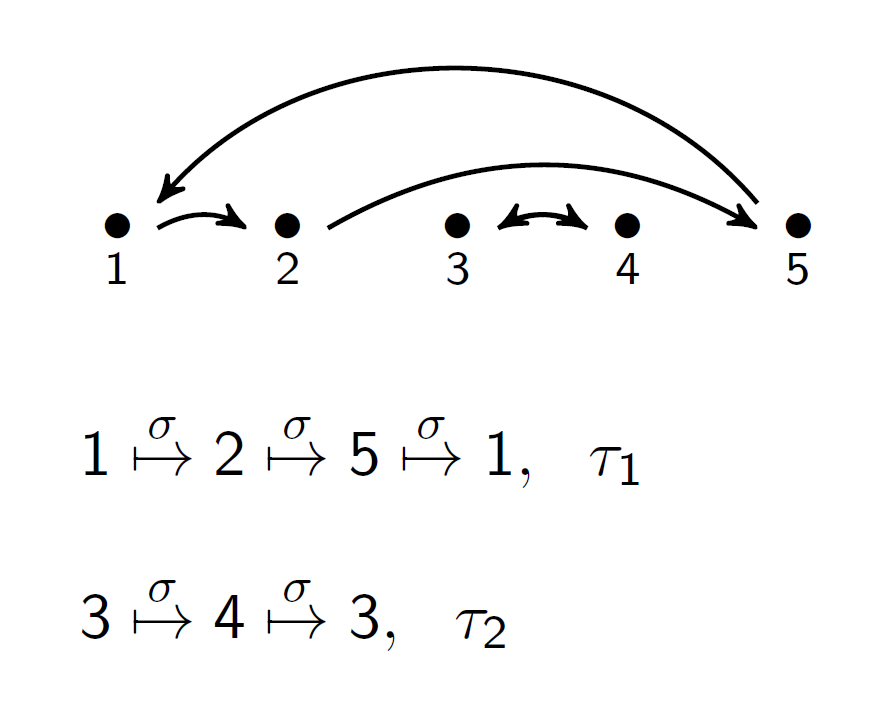
\includegraphics[scale=0.5]{Cycle.png}
    \caption{Example of Cycle}
\end{figure}
\end{center}
In the example of \textit{Figure 1}, $\sigma=\begin{pmatrix}
    1&2&3&4&5\\
    5&1&4&3&2
\end{pmatrix}$, $\sigma=\tau_1\circ\tau_2$, where $\tau_1=\begin{pmatrix}
    1&2&3&4&5\\
    5&1&3&4&2
\end{pmatrix}$, $\tau_2=\begin{pmatrix}
    1&2&3&4&5\\
    1&2&4&3&5
\end{pmatrix}$. $\tau_1$ is 3-cycle, $\tau_2$ is 2-cycle.
We could represent $\tau_1=(1\ 2\ 5)=(2\ 5\ 1)=(5\ 1\ 2)$, i.e.
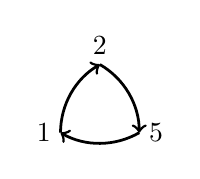
\begin{tikzpicture}[domain=0:3.25]
\draw[->,line width=1] (0.5,0.5*3^0.5) arc (60:0:0.5*2);
\draw[<-,line width=1] (0.5,0.5*3^0.5) arc (120:180:0.5*2);
\draw[<-,line width=1] (0,0) arc (240:300:0.5*2);
\node[left] at (0,0) {$1$};
\node[right] at (0.5*2,0) {$5$};
\node[above] at (0.5,0.5*3^0.5) {$2$};
\end{tikzpicture}
Similarly, we can represent $\tau_2=(3,4)=(4,3)$, i.e.
\begin{tikzpicture}[domain=0:3.25]
    \draw[<->](0,0)--(1,0) node[below] {$$};
    \node[left] at (0,0) {$3$};
    \node[right] at (1,0) {$4$};
\end{tikzpicture}\\
We can find that $\forall x\in \{1,2,3,4,5\}$, $\tau_1^{3}(x)=x, \tau_2^{2}(x)=x$, so we write $\tau_1$ as a \textbf{3-cycle} in $S_5$, $\tau_2$ as a \textbf{2-cycle} in $S_5$.\\

Given $k \geq 2$, a \textbf{k-cycle} in $S_n$ is a permutation $\sigma$ with the property that $\{1,...,n\}$ is the union of two disjoint subsets, $\{1,...,n\}=Y \cup Z $ and $Y \cap Z =\emptyset$, such that\\
1. $\sigma(x) = x$ for every $x \in Z$, and\\
2. $|Y| = k$, and for any$ x \in Y$,$Y = \{\sigma (x), \sigma^2(x), \sigma^3(x)... \sigma^k(x) = x\}$.\\

We say that $\sigma$ \textbf{cyclically permutes} the elements of $Y$ and \textbf{fixes} the elements of $Z$.\\
$\tau_1=(1\ 2\ 5)$ \textbf{cyclically permutes} the elements of $Y=\{1,2,5\}$ and \textbf{fixes} the elements of $Z=\{3,4\}$.\\
$\tau_2=(3\ 4)$ \textbf{cyclically permutes} the elements of $Y=\{3,4\}$ and \textbf{fixes} the elements of $Z=\{1,2,5\}$.\\


\subsection{Disjoint cycles}
Since the sets are cyclically permuted by $\tau_1, \tau_2$ (i.e.$Y$) are disjoint. We call the \textbf{disjoint cycle notation} $\sigma=\tau_1\circ\tau_2=(1\ 2\ 5)(3\ 4)$. (Commute the order is irrelevant)

\subsubsection{Theorem: Every permutation is a union of disjoint
cycles, uniquely.}
Given $\sigma\in S_n$, there exists a unique (possibly empty) set of pairwise disjoint cycles.
\begin{theorem}
Let $X$ be a finite set, the graph of permutation $\sigma\in S_X$ is a union of disjoint cycle.
\end{theorem}
\begin{proof}
Prove by induction:

If $|X|=1$, the graph is circle: 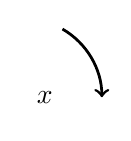
\begin{tikzpicture}[domain=0:3.25]
    \draw[->,line width=1] (0.5,0.5*3^0.5) arc (60:0:0.5*2);
    \node[left] at (0.5,0) {$x$};
    \end{tikzpicture}

\end{proof}








\subsubsection{Proposition 1.3.9: 每个permutation可以由若干个(可能不disjoint的)2-cycles表示}
\begin{proposition}[Proposition 1.3.9.]
    Given $n\geq2$, any $\sigma \in S_n$ can be expressed as a composition of 2-cycles.(not require disjoint)
\end{proposition}
\begin{proof}
    \quad\\
    \begin{equation}
        \begin{aligned}
            (x_1\ x_{k})(x_1\ x_2,...\ x_{k-1}\ x_{k})&=(x_1\ x_2\ ...\ x_{k-1})\\
            (x_1\ x_2\ ...\ x_{k-1}\ x_{k})&=(x_1\ x_{k})(x_1,x_2\ ...\ x_{k-1})\\
            &=\mathbf{(x_1\ x_{k})(x_1\ x_{k-1})(x_1\ x_2\ ...\ x_{k-2})}\\
            &\dots\\
            &=\mathbf{(x_1\ x_{k})(x_1\ x_{k-1})(x_1\ x_{k-2})\dots(x_1\ x_2)}\\
        \end{aligned}
        \nonumber
    \end{equation}
    \end{proof}

\begin{example}[Exercise 1.3.2.]
    Consider $\sigma = (3\ 4\ 8)(5\ 7\ 6\ 9)$ and $\tau = (1\ 9\ 3\ 5)(2\ 7\ 4)$ in $S_9$ expressed in disjoint cycle
    notation. Compute $\sigma\circ\tau$ and $\tau\circ\sigma$ expressing both in disjoint cycle notation.
\end{example}

\begin{equation}
    \begin{aligned}
        &1 \rightarrow \sigma(\tau(1))=\sigma(9)=5;\ 
        2 \rightarrow \sigma(\tau(2))=\sigma(7)=6;\\
        &3 \rightarrow \sigma(\tau(3))=\sigma(5)=7;\ 
        4 \rightarrow \sigma(\tau(4))=\sigma(2)=2;\\
        &5 \rightarrow \sigma(\tau(5))=\sigma(1)=1;\ 
        6 \rightarrow \sigma(\tau(6))=\sigma(6)=9;\\
        &7 \rightarrow \sigma(\tau(7))=\sigma(4)=8;\ 
        8 \rightarrow \sigma(\tau(8))=\sigma(8)=3;\\
        &9 \rightarrow \sigma(\tau(9))=\sigma(3)=4;\\
        \Rightarrow	&\sigma\circ\tau=(1\ 5)(2\ 6\ 9\ 4)(3\ 7\ 8)
    \end{aligned}
    \nonumber
\end{equation}
\begin{equation}
    \begin{aligned}
        &1 \rightarrow \tau(\sigma(1))=\tau(1)=9;\ 
        2 \rightarrow \tau(\sigma(2))=\tau(2)=7;\\
        &3 \rightarrow \tau(\sigma(3))=\tau(4)=2;\ 
        4 \rightarrow \tau(\sigma(4))=\tau(8)=8;\\
        &5 \rightarrow \tau(\sigma(5))=\tau(7)=4;\ 
        6 \rightarrow \tau(\sigma(6))=\tau(9)=3;\\
        &7 \rightarrow \tau(\sigma(7))=\tau(6)=6;\ 
        8 \rightarrow \tau(\sigma(8))=\tau(3)=5;\\
        &9 \rightarrow \tau(\sigma(9))=\tau(5)=1;\\
        \Rightarrow	&\tau\circ\sigma=(1\ 9)(2\ 7\ 6\ 3)(4\ 8\ 5)
    \end{aligned}
    \nonumber
\end{equation}
\begin{example}
    Let $\sigma,\tau \in S_7$, given in disjoint cycle,
    notation by
    $\sigma = (1\ 5\ 4)(3\ 7),
    \tau = (1\ 3\ 2\ 6\ 4)$,
    Compute
    $\sigma^2 ,
    \sigma^{-1} ,
    \tau\circ \sigma$
\end{example}
\begin{equation}
    \begin{aligned}
        &\sigma^2=(1\ 4\ 5),&\sigma^{-1}=(4,5,1)(3,7),\\
        &1 \rightarrow	\tau(\sigma(1))=\tau(5)=5,
        &2 \rightarrow	\tau(\sigma(2))=\tau(2)=6,\\
        &3 \rightarrow	\tau(\sigma(3))=\tau(7)=7,
        &4 \rightarrow	\tau(\sigma(4))=\tau(1)=3,\\
        &5 \rightarrow	\tau(\sigma(5))=\tau(4)=1,
        &6 \rightarrow	\tau(\sigma(6))=\tau(6)=4,\\
        &7 \rightarrow	\tau(\sigma(7))=\tau(3)=2,\\
        \Rightarrow	& \tau\circ \sigma=(1,5)(2,6,4,3,7)
    \end{aligned}
    \nonumber
\end{equation}





\begin{thebibliography}{1}      \bibitem{Long2015Fully}  Christopher J Leininger  \newblock Introduction to Abstract Algebra
    (Draft)  2017.
\end{thebibliography}

\end{document}

\bibliography{reference}
\bibliographystyle{unsrt}